% 75-27(75쪽) — $y=\sin\dfrac{1}{2}x\ (-\pi\le x\le 3\pi)$ 와 두 직선 $y=\pm\dfrac{3}{4}$, 네 점 A, B, C, D(원문 「오른쪽 그림」).
% 스캔 화질이 낮아 TikZ 로 다시 그림. 라벨은 원문 것만: $-\pi$, $\pt{O}$, $\alpha$, $\beta$, $\gamma$, $\delta$, $3\pi$,
% $\pt{A}$, $\pt{B}$, $\pt{C}$, $\pt{D}$, 그래프·직선 이름. $\alpha$ 등의 값은 적지 않는다. 가로축 단위는 $\pi$ 배.
\begin{tikzpicture}[line width=0.6pt, x=0.80cm, y=1.20cm, >=stealth]
  \draw[line width=0.5pt] (-1.65,0.75) -- (3.30,0.75);
  \draw[line width=0.5pt] (-1.70,-0.75) -- (3.35,-0.75);
  \draw[densely dotted, line width=0.35pt] (-1,0) -- (-1,-1);
  \draw[densely dotted, line width=0.35pt] (-0.5399,0) -- (-0.5399,-0.75);
  \draw[densely dotted, line width=0.35pt] (0.5399,0) -- (0.5399,0.75);
  \draw[densely dotted, line width=0.35pt] (1.4601,0) -- (1.4601,0.75);
  \draw[densely dotted, line width=0.35pt] (2.5399,0) -- (2.5399,-0.75);
  \draw[densely dotted, line width=0.35pt] (3,0) -- (3,-1);
  \draw[->, line width=0.7pt] (-1.75,0) -- (5.30,0) node[below=1pt, font=\small] {$x$};
  \draw[->, line width=0.7pt] (0,-1.22) -- (0,1.42) node[left=1pt, font=\small] {$y$};
  \draw[domain=-1:3, samples=200, smooth] plot (\x, {sin(90*\x)});
  \fill (-1,-1) circle (2.2pt);
  \fill (3,-1) circle (2.2pt);
  \node[anchor=south, font=\small] at (-1.0,0.05) {$-\pi$};
  \node[anchor=south east, font=\small] at (-0.04,0.04) {$\pt{O}$};
  \node[anchor=north, font=\small, fill=white, inner sep=0.5pt] at (-0.52,-0.04) {$\alpha$};
  \node[anchor=north, font=\small, fill=white, inner sep=0.5pt] at (0.50,-0.04) {$\beta$};
  \node[anchor=north, font=\small, fill=white, inner sep=0.5pt] at (1.44,-0.04) {$\gamma$};
  \node[anchor=south, font=\small] at (2.52,0.04) {$\delta$};
  \node[anchor=south, font=\small] at (3.02,0.04) {$3\pi$};
  \node[anchor=north west, font=\small] at (-0.48,-0.80) {$\pt{A}$};
  \node[anchor=south east, font=\small] at (0.50,0.80) {$\pt{B}$};
  \node[anchor=south west, font=\small] at (1.50,0.80) {$\pt{C}$};
  \node[anchor=north east, font=\small] at (2.48,-0.80) {$\pt{D}$};
  \node[anchor=south, font=\small] at (1.55,1.02) {$y=\sin\dfrac{1}{2}x$};
  \node[anchor=west, font=\small] at (3.38,0.75) {$y=\dfrac{3}{4}$};
  \node[anchor=west, font=\small] at (3.42,-0.75) {$y=-\dfrac{3}{4}$};
\end{tikzpicture}
